%
% hexagon1.tex -- Koordinaten 
%
% (c) 2019 Prof Dr Andreas Müller, Hochschule Rapperswil
%
\documentclass[tikz]{standalone}
\usepackage{amsmath}
\usepackage{times}
\usepackage{txfonts}
\usepackage{pgfplots}
\usepackage{csvsimple}
\usetikzlibrary{arrows,intersections,math}
\begin{document}
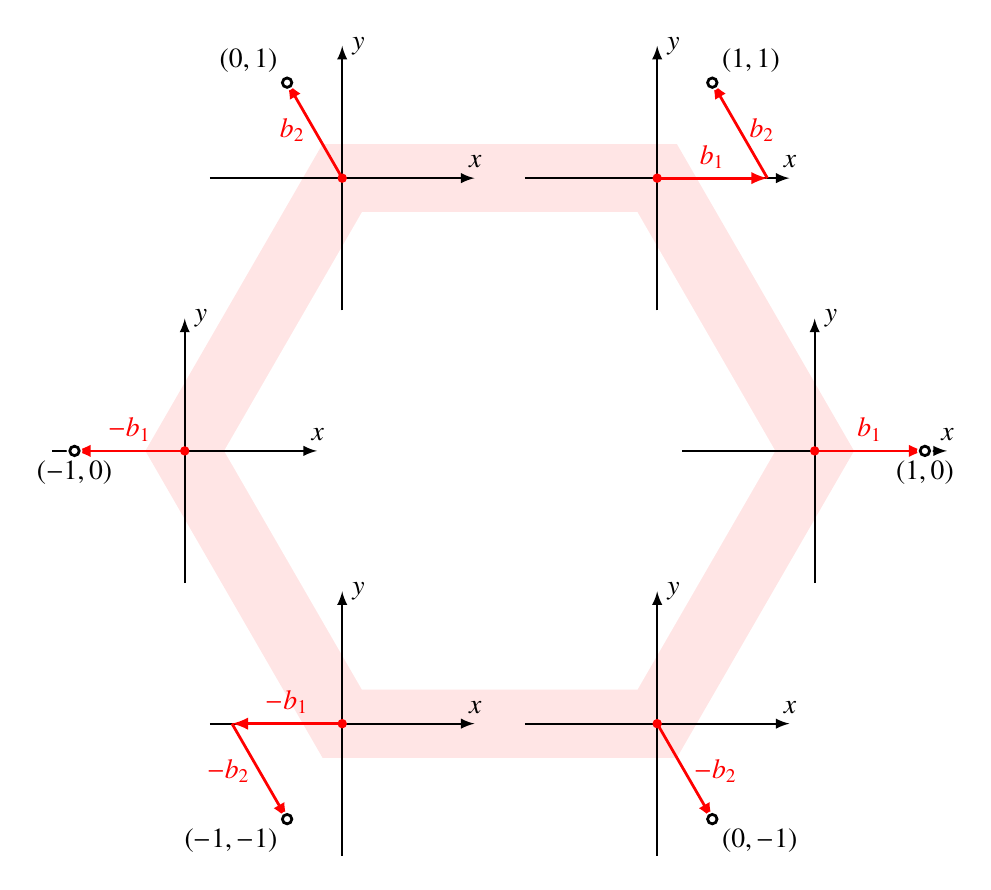
\begin{tikzpicture}[>=latex]

\def\a{1.4}

\def\punkt#1#2{
        \fill[color=white] ({#1},{#2}) circle[radius=0.1];
        \draw[line width=1pt] ({#1},{#2}) circle[radius=0.06];
}

\def\outerradius{4.5}
\fill[color=red!10] 
	(\outerradius,0)--
	({\outerradius*cos(60)},{\outerradius*sin(60)})--
	({\outerradius*cos(120)},{\outerradius*sin(120)})--
	(-\outerradius,0)--
	({\outerradius*cos(240)},{\outerradius*sin(240)})--
	({\outerradius*cos(300)},{\outerradius*sin(300)})--cycle;

\def\innerradius{3.5}
\fill[color=white] 
	(\innerradius,0)--
	({\innerradius*cos(60)},{\innerradius*sin(60)})--
	({\innerradius*cos(120)},{\innerradius*sin(120)})--
	(-\innerradius,0)--
	({\innerradius*cos(240)},{\innerradius*sin(240)})--
	({\innerradius*cos(300)},{\innerradius*sin(300)})--cycle;

\def\achsen{
	\draw[->,line width=0.7pt] ({-1.2*\a},0)--({1.2*\a},0)
		coordinate[label={$x$}];
	\draw[->,line width=0.7pt] (0,{-1.2*\a})--(0,{1.2*\a})
		coordinate[label={right:$y$}];
}

\begin{scope}[xshift=4cm]
	\achsen
	\draw[->,line width=1pt,color=red] (0,0)--({\a},0);
	\node at ({\a},0) [below] {$(1,0)$};
	\punkt{\a*cos(0)}{\a*sin(0)}
	\node[color=red] at ({\a/2},0) [above] {$b_1$};
	\fill[color=red] (0,0) circle[radius=0.06];
\end{scope}

\begin{scope}[xshift=2cm,yshift=3.464cm]
	\achsen
	\draw[->,line width=1pt,color=red] (0,0)--({\a},0);
	\draw[->,line width=1pt,color=red] ({\a},0)--({0.5*\a},{\a*sqrt(3)/2});
	\node at ({0.5*\a},{\a*sqrt(3)/2}) [above right]
		{$(1,1)$};
	\punkt{\a*cos(60)}{\a*sin(60)}
	\node[color=red] at ({\a/2},0) [above] {$b_1$};
	\node[color=red] at ({\a-\a/4},{\a*sqrt(3)/4}) [right] {$b_2$};
	\fill[color=red] (0,0) circle[radius=0.06];
\end{scope}

\begin{scope}[xshift=-2cm,yshift=3.464cm]
	\achsen
	\draw[->,line width=1pt,color=red] (0,0)--({-0.5*\a},{\a*sqrt(3)/2});
	\node at ({-0.5*\a},{\a*sqrt(3)/2}) [above left]
		{$(0,1)$};
	\punkt{\a*cos(120)}{\a*sin(120)}
	\node[color=red] at ({-\a/4},{\a*sqrt(3)/4}) [left] {$b_2$};
	\fill[color=red] (0,0) circle[radius=0.06];
\end{scope}

\begin{scope}[xshift=-4cm]
	\achsen
	\draw[->,line width=1pt,color=red] (0,0)--({-\a},0);
	\node at ({-\a},0) [below] {$(-1,0)$};
	\punkt{\a*cos(180)}{\a*sin(180)}
	\node[color=red] at ({-\a/2},0) [above] {$-b_1$};
	\fill[color=red] (0,0) circle[radius=0.06];
\end{scope}

\begin{scope}[xshift=-2cm,yshift=-3.464cm]
	\achsen
	\draw[->,line width=1pt,color=red] (0,0)--({-\a},0);
	\draw[->,line width=1pt,color=red] ({-\a},0)
		--({-0.5*\a},{-\a*sqrt(3)/2});
	\node at ({-0.5*\a},{-\a*sqrt(3)/2}) [below left]
		{$(-1,-1)$};
	\punkt{\a*cos(240)}{\a*sin(240)}
	\node[color=red] at ({-\a/2},0) [above] {$-b_1$};
	\node[color=red] at ({-\a+\a/4},{-\a*sqrt(3)/4}) [left] {$-b_2$};
	\fill[color=red] (0,0) circle[radius=0.06];
\end{scope}

\begin{scope}[xshift=2cm,yshift=-3.464cm]
	\achsen
	\draw[->,line width=1pt,color=red] (0,0)--({0.5*\a},{-\a*sqrt(3)/2});
	\node at ({0.5*\a},{-\a*sqrt(3)/2}) [below right]
		{$(0,-1)$};
	\punkt{\a*cos(300)}{\a*sin(300)}
	\node[color=red] at ({\a/4},{-\a*sqrt(3)/4}) [right] {$-b_2$};
	\fill[color=red] (0,0) circle[radius=0.06];
\end{scope}

\end{tikzpicture}
\end{document}

